\documentclass[a4paper, 11pt, titlepage]{article}
\usepackage[top=2cm,bottom=2cm,left=2cm,right=2cm]{geometry} 
\usepackage{parskip} 
\usepackage{graphicx}
\usepackage{float}
\usepackage{enumitem}
\usepackage{tabularx}
\usepackage{hyperref}
\usepackage{listings}
\usepackage{xcolor}
\usepackage{array}
\usepackage[export]{adjustbox}

% Define the Alloy language style
\lstdefinelanguage{alloy}{
  keywords={abstract, all, assert, but, check, else, exactly, extends, fact, for, fun, iden, iff, implies, in, let, lone, module, no, none, not, one, open, or, pred, run, set, sig, some},
  sensitive=true,
  morecomment=[l]{//},
  morecomment=[s]{/*}{*/},
  morestring=[b]",
}

% Define the style for Alloy code
\lstdefinestyle{alloyStyle}{
  language=alloy,
  basicstyle=\small\ttfamily,
  keywordstyle=\bfseries\color{blue},
  commentstyle=\color{green!60!black},
  stringstyle=\color{red},
  numbers=left,
  numberstyle=\tiny,
  stepnumber=1,
  numbersep=5pt,
  backgroundcolor=\color{gray!5},
  frame=single,
  tabsize=2,
  captionpos=b,
  breaklines=true,
  breakatwhitespace=true,
  showspaces=false,
  showstringspaces=false,
  showtabs=false,
}

\title{
    CodeKataBattle\\
    \large Software Engineering 2 Project - RASD v2.0
}
\author{
  Mariotti Marco\\
  Personal code: 10939419
}
\date{7 January 2024}

\begin{document}

\maketitle

\tableofcontents

\newpage

\section{Introduction}

\subsection{Purpose}

Today, as the demand for the professional role of programmer is constantly increasing, so is the demand for applications that allow trained programmers as well as hobbyists to grow and hone their skills. Because of this need, \textit{CodeKataBattle} accommodates a growing trend in software development education, where hands-on experience and teamwork play an important role in preparing students for real-world challenges.

The platform operates as a bridge between educators and students, allowing educators to test students from all over the world.
The scope of these challenges is train future programmers using a test-first approach, and in particular training them with peers using 
code kata, which are small programming exercises for which test cases are already provided; in this way, the students can develop succesful routines to solve problems in a specific language without having to worry abbout testing.\newline
\textit{CodeKataBattle} encourages iterative development processes,teaching the importance of continuous improvement to meet all the requests the educator makes.
Instead of more traditional methods, like lectures or online courses, \textit{CodeKataBattle} aims to provide a modern learning experience; in this way students not only reinforce their coding skills but also improve critical aspects such as teamwork, time management, and communication, fundamental skills in many workplaces and vital for success in the dynamic field of software development.

The platform provides users with a user-friendly interface; in particular, the educators can create and manage code kata battles within specific tournaments, that students can participate in, alone or in teams. Educators can upload code katas, set submission deadlines, configure scoring parameters, and give permissions to colleagues to create other battles. 
Also, they can reward the students with badges, defining specific rules to achieve them, adding a competitive gamification element to the experience.
The team score is update every time a team's member push a new commits to their \textit{GitHub} repository (that is created automatically at the beginning of every battle). In this way, both students and educators can monitor the progress of all the teams during the battle.
The tournament rank, that provide insights into individual performance of all the students involved in the tournament, is generated by \textit{CodeKataBattle} summing the battle scores obtained from every battle the student participated in.

\paragraph{The goals of the application are the following:}
\begin{enumerate} [label=G\arabic*:, align=left, leftmargin=*]
    \item Allow students to partecipate in coding tournaments and battles.
    \item Allow students to deliver their solution to the platform.
    \item Allow educators to evaluate team's solution.
    \item Allow students and educators to monitor teams rank during a battle.
    \item Allow students and educatros to monitor tournament score of each student. 
    \item Allow educators to create and manage tournaments and battles.
\end{enumerate}


\subsection{Scope}

In this section, we analyse the world phenomena and the shared phenomena, according to the "World and the Machine" paradigm introduced by M.Jackson and P.Zave. In this context, the Machine is identified with the application to be developed and the world as the real-world environment in which it will be used.

\paragraph{World Phenomena}
\begin{enumerate}[label=W\arabic*:, align=left, leftmargin=*]
    \item A student wants to join a tournament
    \item A student wants to join a battle  
    \item An educator wants to create a new tournament 
    \item An educator wants to create a new battle
\end{enumerate}

\paragraph*{Shared Phenomena}
Shared phenomena are divided according to the controller of the phenomena.

Phenomena controlled by the world:
\begin{enumerate}[label=W\arabic*:, align=left, leftmargin=*]
    \item A student wants to invite other students in a team
    \item An educator wants to grant to other educators the permission to create battles within a specific tournament
    \item A student set up automated workflow through GitHub Actions
    \item A student push a project
    \item An educator wants to manage settings and deadlines for a battle
    \item An educator wants to create a new badge
\end{enumerate}

Phenomena controlled by the machine:
\begin{enumerate}[align=left, leftmargin=*]
    \item [W7:] A student wants to track their progress in a tournament rank
    \item [W8:] Educators and students want to check teams rank during a battle
    \item [W9:] Educators and students want to check active tournaments
    \item [W10:] Educators and students want to check collected badges
    \item [W11:] The app notifies all the students of the creation of a new tournament
    \item [W12:] The app notifies all the students in a tournament of the creation of a new battle
    \item [W13:] The app creates a GitHub repository and send the link to all the team's members
    \item [W14:] The application assigns badges according to their rules
\end{enumerate}
\subsection{Definitions, Acronyms, Abbreviations}
\textbf{Definitions:}
\begin{itemize}
    \item \textbf{CodeKataBattle:} The software to be developed.
    \item \textbf{Student:} The participant in one or more tournaments and battles
    \item \textbf{Educator:} The creator of one or more tournaments and battles
    \item \textbf{Tournament:} A competition composed of multiple battles
    \item \textbf{Battle:} A contest of multiple teams to create a project that satisfies all the tests
\end{itemize}
\textbf{Acronyms:}
\begin{itemize}
    \item \textbf{CKB:} CodeKataBattle
\end{itemize}
\subsection{Revision history}
\begin{itemize}
    \item v1.0 : First version of the document released on December 22, 2023.
    \item v2.0 : Make minor adjustments to the document's formatting and address typing errors. Enhance the functional requirements section by incorporating additional details. Expand the product function section by subdividing existing subsections into more specific cases and providing more comprehensive descriptions for some of these cases.
\end{itemize}
\subsection{Reference Documents}
\begin{itemize}
    \item The specification document ”Assignment RDD AY 2023-2024”.
\end{itemize}
\subsection{Document structure}
This document is composed of the chapters described below.
\begin{enumerate}
    \item The first chapter contains a brief introduction to the problem with the goals of the project.
It also contains analysis of world and shared phenomena, followed by a description of the
document as a whole.
    \item The second chapter contains a description of the system to be. Here are presented scenarios, a
class diagram of the system, some statecharts and a list of domain assumptions and dependencies
made for the project.
    \item The third chapter contains a description of the requirements of the system. Here, use cases are
presented with their diagrams. Then, functional and non-functional requirements are presented
and mapped on goals.
    \item The fourth chapter contains a formal analysis made with Alloy.
    \item The fifth chapter contains the description of the effort spent by the group members.
    \item The sixth chapter contains the eventual used references.
\end{enumerate}

\newpage

%***************************************************************%
%************************** CHAPTER 2 **************************%
%***************************************************************%


\section{Overall Description}

\subsection{Product perspective}
In the first part of this section, we will analyse some scenarios involving the usage of CKB.
\begin{itemize}
    \item \textbf{User Registration on CKB:} 
    Jamie, a computer science student, decides to check out the CodeKataBattle application under the
    recommendation of one of his professors, to improve his programming skills for one of his university courses.
    Through his laptop, he opens the CKB homepage and after reading the description on the CKB website, decides to sign up to the platform.
    He cicks on the "sign up" button on the homepage and he is redirected to the sign up form, through which he inserts all required personal data,
    like name, surname, email, a username and password. After linking his GitHub profile, he successfully created an account on the CKB platform.
    
    \item \textbf{Educator Creates a New Tournament:} John, a computer science professor, logs into the CKB application because he has decided to create
     a challenging code kata tournament for the students of his class as part of the final mark for his course. He clicks on "Create new tournament"
      banner, enters the required data and customizes all aspects of the tournaments according to his needs, like the tournament description and subscription deadlines. Lastly,
       John decide to give permission to other collegues to create new battles for the partecipants.

    \item \textbf{Educator Creates a New Battle:} Sarah, a computer science professor, decides to create a new battle for one of the tournaments she manages.
    To do so, she opens the CKB appliation, chooses one of the tournaments and clicks on the "create a battle" button. Because of the wide range of customization the application offers, she is able to organize and set the 
    battle in the best possible way to accomodate her students' learning needs. After customizing the battle description and deadlines, she uploads the Code Kata including its test cases and build automation scripts. Then,
    she is able to customize the parameters used for evaluation and computation of the final score. Other than configuring the standard timeliness and functionality parameters, Sarah is also able to choose which aspects will be 
    analyzed for the evaluation of the quality parameter, and which weight they will have on the final score automatically computed by the system.

    \item \textbf{Student Joins a Code Kata Battle:} Kelly logs into the CKB application after receiving a notification
     for the creation of a new battle in the tournamet in which she is involved. After reading the battle description and all related details,
      Kelly decides to form a team to participate in this battle. In the team creation section, Kelly selects the number of teammates she want
       for the team (ensuring that respect the minimum and maximum value for the battle) and sends an invitation
        to some of her friends, waiting for thir response. In the meantime, she also receives a request by another user to join her team , which she decides to decline.
        After her team is complete, her team officially joins the battle.

    \item \textbf{Student Submits Code Solution:} Jordan, a prticipant of a Code Kata battle, after finishing writing and modifying the code for his project locally on his IDE of choice,
    decides to push his work on the team's GitHub repository, eager to know the result. This action triggers an automated 
    analysis of the code (considering factors such as functionality, timeliness, and code quality as set by the educator which created the battle). 
    After the analisys is finished, the team's score is dynamically updated and dispayed on the rank of the battle on the platform.

    \item \textbf{User Visualizes Real-Time Battle Rank:} Taylor logs into the CKB application to visualize the position
     of her team in the battle they are involved. She navigates to the real-time battle rank section and
      the rank with all the teams's scores appears, providing a clear rappresentation of the situation
       of the team in the battle and allowing her to plan how to manage their work accordingly. 
       Scrolling the leaderbord she finds out that they are in the middle of the list, so they need to put 
       much more effort in the competition to obtain a good score.

    \item \textbf{User Receives Final Battle Rank Notification:} Mark is impatient to know the final 
    result of the battle he has participated in the past weeks. Some days after the battle concludes, Mark receives
     a notification from CKB application. Navigating in the website, on the tab of the tournament, Mark visualize the 
     final rank, understanding the level of his coding skills and that he still has a lot to improve to 
     reach the top.

    \item \textbf{Student Accumulates Tournament Scores:} Pat logs into CKB to visualize his personal score in
     the tournament he is involved. Pat navigates to the tournament scores section, visualizing his and other 
     partecipants scores; in this way, Pat can see clearly his situation in the tournament and have a a clear view  
     of all the other partecipants.

    \item \textbf{Educator creates a badge:} Morgan, an educator using CKB to challenge their students, decides to 
    make the challenge more fun and competitive through the gamification feature offered by the platform. During the tournament
    creation phase, Morgan decides to create some badges associated to the tournament, which will be assigned to students who fullfill their requirements. 
    In particular, he decides to create a new badge named "Unity is strength" to reward the collaboration between students.
    In the badge creation window within the tournament creation, he sets the name of the badge and the rule to achieve it:
    $ {team\_memebers} > 3 $
, selecting \textit{team\_members} in the list of available attributes to create rules for badges. 
    In this way all the students that partecipate in a battle with a team of four or more members receive this badge.
\end{itemize}
After the presentation of the above scenarios, we can formalize a \textbf{UML class diagram} for our system. 

\begin{figure}[h]
    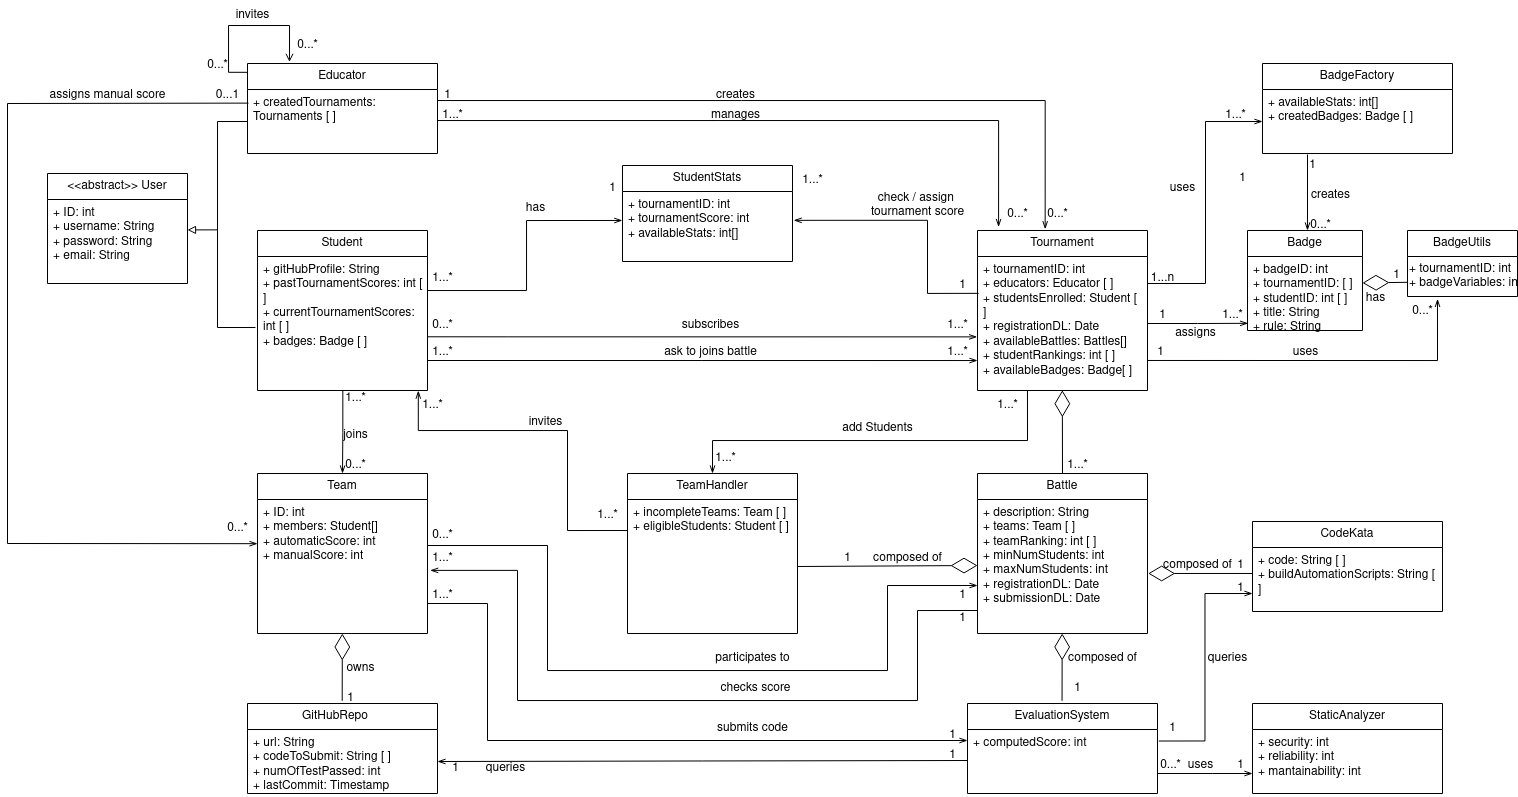
\includegraphics[width=1\textwidth]{images/UML_231221.png}
    \caption{CKB Platform UML Class Diagram}
    \label{fig:CKB_uml1}
    \centering
\end{figure}

Here are some notes regarding the most important entities of the diagram.
\begin{itemize}

    \item The \emph{User} abstract class is specialized into \emph{Student} and \emph{Educator}. Educators are the users who can create new Tournaments and Battles, while Students can partitipate to a Tournament, compete in Battles and receive Badges.
    
    \item The educator creates a Tournament by instantiating a \emph{Tournament} class. This class is composed of different \emph{Battle} classes, each one representing a battle created by an educator. The \emph{Battle} class itself is composed of a \emph{CodeKata} class containing the actual code of the battle, a \emph{TeamHandler} class which is responsible for handling the creation of teams that will participate to the battle, and an \emph{EvaluationSystem} class, used to compute the score of each team for the current battle. 
    
    \item Each students subscribed to a Tournament has a \emph{StudentStats} class associated to. This class contains 
    \begin{itemize} 
        \item the tournament score for the corresponding student
        \item the \emph{availableStats} list, containing all the statistics provided by the CKB platform, tailored for the current turnament. This list will be used to gather the necessary variables in order to assign Badges to each student.
    \end{itemize}

    \item Whenever a student subscribed to a tournament wants to join a battle, he queries the \emph{Tournament} class, which contains the list of available battles. In order to take part to the battle, the student has to either create a team or join an existing one. The \emph{Tournament} class adds the student to the \emph{TeamHandler} class associated with the battle picked by the student. \emph{TeamHandler} contains a list of students that can be invited (which is a list of all students registered for the tournament, excluding students who are part of a complete team for the current battle) and a list of the incomplete teams. Note that a student part of an incomplete team can still be invited to or join another team. Whenever a team contained in \emph{TeamHandler.incompleteTeams} is completed, it is moved to \emph{Battle.teams} and its members are removed from \emph{TeamHandler.eligibleStudents}. Students part of complete teams cannot switch to another team anymore.
    
    \item A tournament must have at least one battle available. If at the battle registration deadline no team has joined it, the battle is cancelled.

    \item Every time a team participating to a battle commits to the GitHub repository, the code is also submitted to the \emph{EvaluationSystem} class, which compute the automatic score for that specific team by querying the \emph{GitHubRepo} and \emph{codeKata} classes in order to evaluate the functional aspect and also the timeliness (\emph{GitHubRepo.lastCommit} attribute serves this purpose). The quality aspect of the score (security, reliability, mantainability) are evaluated using the \emph{StaticAnalyzer} class, that exploits the API of Static analisys tools such as \href{https://www.sonarsource.com/products/sonarqube/}{SonarQube} to compute this portion of score. Ultimately, the manual portion of the code can be assigned directly by the \emph{Educator} class. The \emph{Battle} class retrieves the score from each team to compute the real time battle ranking.
    
    \item At the end of the battle, every team component has its own \emph{StudentStats.tournamentScore} updated.

    \item The educator can create new Badges and add them to the current Tournament (the \emph{Tournament} class has an \emph{availableBadges} attribute). The process of creating a badge is handled through the \emph{BadgeFactory} class: starting from a list of statistics provided by the CKB platform, the Educator can compute the required badge variables and the correspondig badge rules. Every \emph{Badge} class has a \emph{BadgeUtils} class associated to, which contains a list of the badge variables and the method to compute them. 
    
    \item The assignment of badges is managed by the \emph{Tournament} class, as it can access the statistics of all students (contained in \emph{StudentStats.availableStats}) and all badge variables (contained in \emph{BadgeUtils.badgeVariables}). For every Badge, the \emph{Tournament} class:
    \begin{itemize}    
        \item retrieve how to compute the badge variables from the \emph{BadgeUtils} class
        \item retrieve the statistics of each student
        \item compute the badge variable for each student
        \item assigns the badge
    \end{itemize}
\end{itemize}

\newpage

Now we will analyze the behaviour of some object from the UML class diagram. In particular, we will use \textbf{state diagrams} to display the changes the object is subjected to over time.

\vspace{0.5cm}

The state diagram below shows the behaviour of the \emph{User} object through the entire charging process. Please note that an user can decide to subscribe to CKB either as \emph{Educator} or as \emph{Student}. 

\begin{figure}[h]
    \includegraphics[width=1\textwidth]{images/statechart_userRegistration.png}
    \caption{User registration state diagram}
    \label{fig:CKB_sc1}
    \centering
\end{figure}

The state diagram below shows the process of joining a \emph{Battle}. Please note that a student must be subscribed to the tournament hosting the battle in order to join it. Also, as long as the chosen \emph{Team} is not completed, the student can leave it for another one. Lastly, if the battle subscription deadline expires and the Student is in an incomplete team it cannot participate to the battle.

\begin{figure}[h]
    \includegraphics[width=1\textwidth]{images/statechart_battleRegistration.png}
    \caption{Battle registration state diagram}
    \label{fig:CKB_sc2}
    \centering
\end{figure}

\newpage

The state diagram below shows the process of updating the \emph{Real Time Battle Score}. The process is triggered every time there is a commit to the Team's repo. When the battle deadline expires, the \emph{Automatic Score} is finally computed and we enter the consolidation phase in which the \emph{Manual Score} is assigned by an educator (if required). 

\begin{figure}[h]
    \includegraphics[width=1\textwidth]{images/statechart_battleScore.png}
    \caption{Battle score computation state diagram}
    \label{fig:CKB_sc3}
    \centering
\end{figure}

\subsection{Product Functions}
In this section, the main functionalities of CKB are presented and described in-depth.
\begin{itemize}
    \item \textbf{Creation of a Tournament by an Educator:} CKB must provide already registered educators the possibility to create a personalized tournament in a simple way. 
    On the main menu, they need to press the "create new tournament" tab and, in the newly opened window, they should specify all the 
    fundamental information, such as the tournament name, description, and subscription deadline. Optionally, the system also allows educators to set an icon for the tournament. After customizing all mandatory settings, the tournament creation function should allow 
    educators to choose whether to add collectible badges to the tournament. This function must be optional, as a tournament can be fully functional without badges.
    In case educators want to add badges to the tournment, an appropriate customization window should be provided to the user, in order to allow them to have a comprehensive
    and clear view of all parameters available to create rules.The system should allow the user to to create multiple badges within the same tournament. For each one, the application should
    provide functionalities to set a name, a brief description and an optional icon. Then, an arbitrary number of rules can be added, in the following form:
    \[[system\_parameter] \leq,<,=,>,\geq [value,true,false] \]
    in which true and false are only available for boolean parameters, while value can be a static value set by the educator or a dynamic value generated by CKB, for example \textit{max-tot-commits}. Moreover, the user should be allowed to choose the relationship between rules with \textit{and} and \textit{or}
    logical operators, by writing simple logical expressions using previously defined rules and parenthesis, if needed:
    \begin{center}
        \textit{(rule1 or rule2) and rule3}
    \end{center}
    Rules will be evaluated and checked by a validator included in the badge creation functionality, in order to establish if the logical expression can be actually fulfilled and students can actually
    obtain the badge.
    
    \item \textbf{Manage Tournament:} CKB must allow educators to manage tournaments they have created. Each educator must be provided with
    the list of tournament they have created, and for which they are allowed to exploit all fuctionalities as administrators, and the list of tournaments to which they
    have been invited to collaborate. For created tournaments, educators must be allowed to invite other educators as collaborators, by going in the tournament management section and choosing the
    "invite educator" functionality. The invited educator should be allowed to accept or deny the request.\\ In the tournament management section, educators should also be able to view the current status of the tournament rank and the status of all battles within the tournament.
    Educators that are also creators of a tournament must be allowed to close the tournament whenever they seem fit, as long as there are no active battles in the tournament. This function must not be provided to 
    educators which have been invited to manage a tournament.  

    \item \textbf{Creation of a Battle by an Educator:} CKB must provide already registered educators the possibility to create a new battle 
    within tournaments they manage. By clicking the "create battle" tab, a window opens, and the educator is provided an interface through which they can enter all the 
    necessary descriptive information, such as the name of the battle and a description of the challenge. After setting preliminar informations, the educator is asked to upload the software project (including the test cases and the 
    automatic scripts). The educator should also be allowed to set requirements for the creation of teams, like the minimum and maximum number of members for each group. They also need to set two different deadlines, one 
    for the subscription to the battle by students and the other for the end of the battle.
    Lastly, the aplication should provide all necessary functions to customize the evaluation system for the battle. The automatic evaluation system takes into account three different scoring parameters. Each parameter will have a weight on the final score
    set between 0 and 1, also customizable by the educator, and the final sum of all weights will be 1, as to obtain a total score of maximum 100 points. Available parameters are the following
    \begin{itemize}
        \item \textit{Functional.} This parameter measures the number of test cases passed out of all test cases. The maximum number of points that can be obtained through this parameter will be equally distributed among all test cases. 
        As an example, if the functional parameter allows students to score a maximum of 30 points and the project provides 10 test cases, each test case passed will allow
        students to score 3 points. The only customization option provided by this paramter is its weight.
        \item \textit{Timeliness.} This parameter evaluates how much time was spent to complete the project with relation to the registration deadline. After half of the available days are passed, points will be equally 
        distributed among the remaining days available to complete the project and will be progressively subtracted to the total number of obtainable points each time a push is executed in a new day. Educators can choose the starting time from which points will be 
        detracted, other than the weight of this parameter on the total score. 
        \item \textit{Quality}. Quality level of the sources can be evaluated according to multiple parameters, such as security, reliability and mantainability. The educator must be allowed to choose how many parameters to consider as they deem appropriate, to do so the 
        \item application must provide a toggle feature. The application must be connected through appropriate APIs to any third party application, such as \textit{SonarQube}, that is able to provide static analisys of code based on the selected parameters.    
    \end{itemize} 
    Other than the previously described parameters, the educator must indicate whether they want to provide a manual evaluation, whose points will contribute to the final score of the team. This optional evaluation will also have a weight that must
    conform to the previously stated rules.
    
    \item \textbf{Allow a Student to Join a Tournament:} CKB must allow students to browse and choose a tournament to join. To do so, a list of all ongonig tournaments must be available to all students subscribed to the platform, equipped with 
    appropriate search and sort features to allow students to find the best tournament according to their skill level and their interests. On the tournament overview page, a join option must be provided if the tournament is still open for subscriptions.
    
    \item \textbf{Allow a Student to Join a Battle:} CKB must provide the students involved in a tournament with the opportunity to join a battle by different means. 
    Any student that wants to join a battle must create or join an existing team first, according to the rules stated in the battle desciption. For this reason, different features are provided to the student to make the process of joining a battle as flexible as possible.
    \begin{itemize}
        \item \textit{Create a new team.} Each student is allowed to create their own team for any battle. This feature allows the student to choose a name for the team and the number of members. Within the creation context,
        if the team has more than one member (including the creator), the student can already send invites to other students subscribed to the same tournament by searching their username in a search bar. This feature must also be available after the team creation process is completed: 
        incomplete teams are displayed in the battle overview page until they can join the battle. 
        Any team member can send join invites to other students within the tournament. If the team has only one member and is compliant with battle rules, upon completing the 
        team creation process the team immediately joins the battle.
        \item \textit{Join an existing team}. Upon visualizing the battle overview page, students are provided with the list of teams that have not reached ther maximum number of members yet. Students must be allowed to choose any team among the list,
        to visualize the team detailes, including the maximum number of members and current members, and must be allowed to send a join request to the team they prefer. At the same time, any member of a team that receives a join request is provided with the option to accept or decline a request. 
        Once a team member performs one of those actions, other members cannot override that action.   
        \item \textit{Quit team.} Students who are members of incomplete teams should also be allowed to quit their team. This feature must only be available for teams that have not joined the battle yet.
        If the only team member of a team decides to quit, the team is deleted. 
    \end{itemize}
    Join requests by students and join invites by teams can be acceped or denied. As soon as a team reaches its maximum number of members, it is removed from the list of incomplete teams and joins the battle. At this point all information 
    about the team cannot be edited, and team members cannot quit the team.
    \item \textbf{Allow Users to Check Rankings:} CKB applications provides a ranking system for both tournaments and battles. 
    \begin{itemize}
        \item The tournament rank is based on the personal score assigned to each student. Each time a student completes a battle and obtains a score, this score is summed to their personal score.
        For this reason, the battle rank is updated each time a battle is officially closed. The tournament overview page must allow both educators and students to check the current tournament rank.
        \item The battle rank is based on the progressive score obtained by each team during a battle. Each time a push is executed ont he GitHub repository of a team, a new evaluation is performed and the team score is updated, thus updating the rank.
        The battle rank must be available in the battle overview page, and both students and educators must be allowed to check it whenever they seem fit. 
    \end{itemize} 

    \item \textbf{Allow Students to be Notified of Relevant Actions:} CKB must provide a notification system to inform students of relevant actions and events. Multiple scenarios 
    can trigger notifications, which will be displayed in an inbox on the student's account and sent by e-mail, to the address specified during the registration process. The e-mail notification can be optional, users
    should be provided with the function to toggle them on or off. Actions that should trigger notifications are the following:
    \begin{itemize}
        \item \textit{Creation of a tournament.} Each time a tournament is created, all students should receive a notification that a new tournament is available.
        \item \textit{Expiration of battle subscription deadline.} When the battle subscription deadline expires, all subscribed students will receive a notification with the link of the GitHub repository for the project.
        \item \textit{A battle is officially closed.} After the final battle rank is computed, all subscribed students will receive a notification informing them that the final rank is available.
        \item \textit{Closing of a tournament.} When an educator decides to close their tournament, all subscribed students will be notified, as the final rank and assigned badges (if provided) are available.
        \item \textit{Join requests or invites.} Whenever educators are invited to join a tournament, students are invited to join a battle or receive a join request for their team, they will be notified.
    \end{itemize}
    Student should also be able to choose for which one of these actions they want to receive real-time notifications, or if they prefer a daily or weekly recap. 
    
\end{itemize}
\subsection{User Characteristics}
In our CKB system, the following type of users are considered:
\begin{itemize}
    \item \textbf{Unregistred student:} students that are not yet register on CKB. They need to create an account to access the service offered by CKB.
    \item \textbf{Registered student:} students that have an account on CKB. They can use all the functionality offered by CKB for students, for example partecipates at a new tournament.
    \item \textbf{Unregisters educator:} educators that are not yet register on CKB. They need to create an account to access the service offered by CKB.
    \item \textbf{Registerd educator:} educators that have an account on CKB. They can use all the functionality offered by CKB for reducators, for example create a new tournament .
\end{itemize}
\subsection{Assumptions, Dependencies and Constraints}
\textbf{Domain Assumptions:}
\begin{enumerate}[label=D\arabic*:, align=left, leftmargin=*]
    \item Users enters correct information regarding themself.
    \item Every user has an eletronic device with internet access.
    \item Educators provide a description of the tournament they are creating.
    \item Students joining battles have valid accounts.
    \item Students can partecipate on multiple tournaments at the same time.
    \item Students can partecipate on multiple battles at the same time, also in the same tournament.
    \item A tournament consists in different battles, and each battle can be on different programming language.
    \item The students that partecipate in a battle fork the GitHub repository of the team and set up an automated workflow through GitHub Actions.
    \item The battle rank updates after a commit during the battle.
    \item Personal tournament scores sums all the scores obtained by a students in the code kata battles within a tournament.
    \item Educators define accurate scoring parameters for code katas battles.
    \item Notifications are delivered promptly to participants after a new tournament or battle is created, or when a battle finish.
    \item Automated evaluation criteria, including functional aspects, timeliness, and source code quality, produce consistent results.
    \item Gamification badges have precise rules to satisfy to be assign to a student.
    \item Gamification badges rules refers on existing variables.
\end{enumerate}
\textbf{Dependencies:}
\begin{enumerate}[label=De\arabic*:, align=left, leftmargin=*]
    \item CKB integration with GitHub relies on its stability to works properly.
    \item Users depend on stable and secure internet connections to participate in code kata battles.
    \item Users depend on modern web browsers that support the website.
\end{enumerate}

%***************************************************************%
%************************** CHAPTER 3 **************************%
%***************************************************************%

\section{Specific Requirements}

\subsection{External Interface Requirements}

\subsubsection{User Interfaces}
The user interface of CKB must satisfy the needs of both educators and students. The main user interface
is a website, that must be available from any type of ”common” device (like personal computers,
tablets and smartphones). In a reasonable way, it is possible to assume that most educators will
use an office dekstop while students might want to use also a mobile phone, so also a mobile-friendly version of the user interface must be be implemented.


\subsubsection{Hardware Interfaces}
CKB is a web-based system. Hence, in order to access it, a generic device, like personal computers, laptops, tablets, and smartphones, with an internet
connection is needed.

\subsubsection{Software Interfaces}
To work properly, the CKB system relies on some external softwares:
\begin{itemize}
    \item  GitHub provides an API that enables the system to generate new repositories for each team involved in a battle.
    \item  The system integrates with a static analysis tool, that provides an API for incorporating the static analysis of projects, contributing to the automatic score of the team.
\end{itemize}

\subsection{Functional Requirements}
In this section are presented the most relavant use cases for the CKB application.
Each use case is illustrated through the associated sequence diagram, while all uses cases are grouped and presented together in
the use case diagram. Entry conditions and exit conditions are the conditions that must hold for the actor to enter and exit the use case.  

\subsubsection*{UC1: Student registration}

\begin{center}
    \begin{tabularx}{\linewidth} {|c|X|}
        \hline
        Actors & Student\\
        \hline
        Entry condition & 
            A user wants to register on the CKB platform as a student.\\
        \hline
        Event flow & 
        \begin{enumerate}
            \item The student opens the CKB home page and clicks on the sign up/sign in button.
            \item The student chooses the "sign up as a student" option and the registration form is loaded.
            \item The student fills in the form with their personal data and account credentials, such as name, surname, e-mail, password and username.
            \item The CKB platforms reteives the request and checks if the e-mail is valid and the password is conform to securety standards.
            \item The student is asked to link their CKB account to their GitHub account.
            \item The student is redirected to the GitHub login page.
            \item The student inserts their GitHub credentials and logs into their account.
            \item The student is redirected to the CKB registration page.  
        \end{enumerate}\\
        \hline
        Exit condition &
            The student is successfully registered to the CKB platform and correctly 
            linked their GitHub account.\\ 
        \hline
        Exception & 
        \begin{enumerate}
            \item The student can't complete the registration process due to multiple reasons:
           \begin{itemize} 
            \item The credentials submitted are not adequate.
            \item The e-mail is not well formatted.
            \item The e-mail submitted is already used by another account. 
            \item The username is already used by another account.
            \item The password used is not strong enough according to the platform's security standards.
            \item The user fails to log in their Github account because the credentials are wrong.
           \end{itemize}
           \item The platform fails to retreive the GitHub login page. The user is invited to refresh the page and try again.  
           \item Internet connection is lost during any phase before the completition of the registration process.
        \end{enumerate}\\
        \hline
        
    \end{tabularx}
\end{center}
\newpage
\begin{figure}[h!]
    \centering
    \includegraphics[width=0.8\textwidth]{images/student registration_s.png}
    \caption{Student registration}
    \label{fig:seq_diag_student_reg}
    
\end{figure}

\clearpage 

\subsubsection*{UC2: User login}
\begin{center}
    \begin{tabularx}{\linewidth}{|c|X|}
    \hline
    Actors & User\\
    \hline
    Entry condition & a user \(student or educator\) wants to log in the CKB platform.\\
    \hline
    Event flow & \begin{enumerate}
        \item The user opens the CKB application and asks to log in.
        \item The CKB application displays the login page.
        \item The user inserts their account credentials.
        \item The user logs in the platform.
    \end{enumerate}\\
    \hline
    Exit condition & The user logs in the CKB application.\\
    \hline
    Exception & \begin{itemize}
        \item The user inserts wrong credentials. In this case an error message is displayed and the user is incvited to try again.
        \item An error occurs during the authentication process.
        \item Internet connection is lost before all oeprations are completed.
    \end{itemize} \\
    \hline
    \end{tabularx}
\end{center}

\begin{figure}[h!]
    \centering
    \includegraphics[width=0.50\textwidth]{images/user_login_s.png}
    \caption{A user logs in the CKB platform}
    \label{fig:seq_diag_user_login}
    
\end{figure}

\clearpage

\subsubsection*{UC3: Join a tournament}

\begin{center}
    \begin{tabularx}{\linewidth} {|c|X|}
        \hline 
        Actors & Student\\
        \hline 
        Entry condition &
            A student wants to join one of the open tournaments.\\
        \hline 
        Event Flow &
        \begin{enumerate}
            \item The student opens the CKB home page and logs in.
            \item The student clicks on the "View active tournaments" button.
            \item The list of active tornaments is displayed.
            \item The student filters the list to see which tournaments are open to join.
            \item The student sends a request to join the tournament by clicking on the join button.
            \item The student is subscribed to the tournament.
        \end{enumerate}\\
        \hline 
        Exit Condition & The student is successfully subscribed to the tournament.\\
        \hline 
        Exception & 
        \begin{itemize}
            \item The student clicks on the join button seconds before the subscription deadline expires, in this way the platform does not have 
            enough time to complete the subscription process before the deadline.
            \item There are no open tournaments available to join.
            \item Internet connection is lost before completing the operation.
        \end{itemize} \\
        \hline
    \end{tabularx}
\end{center}

\begin{figure}[h!]
    \centering
    \includegraphics[width=0.7\textwidth]{images/join_tournament_s.png}
    \caption{Student joins a tournament}
    \label{fig:seq_diag_tournament_join}
    
\end{figure}

\clearpage

\subsubsection*{UC4: Create a team}

\begin{center}
    \begin{tabularx}{\linewidth} {|c|X|}
        \hline 
        Actors & Student\\
        \hline 
        Entry condition & The student wants to join a battle by creating a new team.\\
        \hline 
        Event Flow &
        \begin{enumerate}
            \item The student asks the platform to display the list of available battles 
            for a certain tournament.
            \item The student selects a battle.
            \item The CKB application opens the battle overview page, displaying its details.
            \item The student clicks on the button to join the battle.
            \item The CKB application displays the "join battle" page, where the student is asked to coose between creating a new team or joinin an 
            existing one.
            \item The student decides to create a new team.
            \item The student fills the form with the team settings, including the number of participants.
            \item If the team has only one participant, the team is registered to the platform and joins the battle immediately.
            \item If the team has more than one participant, the team is stored by the TeamHandler until the team is complete.
        \end{enumerate}\\
        \hline 
        Exit Condition & 
        The student creates a team and joins the battle.
        The student creates a team and is put in the waiting list.\\
        \hline 
        Exception & 
        \begin{itemize}
            \item The application fails to retreive the list of available battles.
            \item The application fails to load the batttle overview page.
            \item The application fails to upload the team settings.
            \item The application fails to register the team.
            \item The internet connection is lost before the last operation si completed.
        \end{itemize}\\
        \hline
    \end{tabularx}
\end{center}

\begin{figure}[h!]
    \centering
    \includegraphics[width=1.0\textwidth]{images/create_team_s.png}
    \caption{Student creates a team and joins a battle}
    \label{fig:seq_diag_create_team}
    
\end{figure}

\clearpage

\subsubsection*{UC5: Join a team}

\begin{center}
    \begin{tabularx}{\linewidth} {|c|X|}
        \hline 
        Actors & Student\\
        \hline 
        Entry condition &
        The student wants to join a battle by joining an already existing team\\
        \hline 
        Event Flow &
        \begin{enumerate}
            \item The student asks the platform to display the list of available battles 
            for a certain tournament.
            \item The student selects a battle.
            \item The CKB application opens the battle overview page, displaying its details.
            \item The student clicks on the button to join the battle.
            \item The CKB application displays the "join battle" page, where the student is asked to choose between creating a new team or joinin an 
            existing one
            \item The student decides to join an existing team, so the platform shows them the list of incomplete teams.
            \item The student selects a team and sens a join request.
            \item If the team accepts the request, the student is added to the team.
            \item If the team reaches the total number of participants specified in its settings, it automatically joins the battle.
            \item If the team is still incomplete, it remains in the waiting list. 
        \end{enumerate}\\
        \hline 
        Exit Condition &
        \begin{itemize}
            \item The student is added to the team and the team is still incomplete.
            \item The team is complete and it joins the battle.
            \item The request is rejected. 
        \end{itemize}
        \\
        \hline 
        Exception & 
        \begin{itemize}
            \item The application fails to load the requested views and pages
            \item The request is not accepted nor rejected before the battle subscription deadline expires. In this case, if the team is still incomplete, it cant join the battle.
            \item If the team accepts other requests or successfully invites other students before the deadline expires, it can still join the battle. If the team joins the battle before answering the request, the request is considered as rejected.
            \item Internet connection is lost before all operations are completed.
        \end{itemize}\\
        \hline
    \end{tabularx}
\end{center}

\begin{figure}[h!]
    \centering
    \includegraphics[width=1.0\textwidth]{images/join_existing_team_s.png}
    \caption{Student joins an existing team for a battle}
    \label{fig:seq_diag_join_team}
    
\end{figure}

\clearpage

\subsubsection*{UC6: Invite a student to join the team}

\begin{center}
    \begin{tabularx}{\linewidth} {|c|X|}
        \hline 
        Actors & Student\\
        \hline 
        Entry condition & A team member invites a student to join their team\\
        \hline 
        Event Flow &
        \begin{enumerate}
            \item A student (team member) asks the platform to show the list of students
             subscribed to the tournament but that are not part of any team yet.
             \item The student selects another student from the list and send them an invitation request to join their team.
             \item If the receiving student accepts the request and the team is not complete yet, they're added to the team.
             \item If the team is then complete, it automatically joins the battle. Otherwise, it remains in the waiting list.
             \item If the request is rejected, team members are notified and the student is not added to the team. 
        \end{enumerate}\\
        \hline 
        Exit Condition &
        \begin{itemize}
            \item The request is accepted, the team is complete and joins the battle.
            \item The request is accepted, the team is incomplete and is kept in the waiting list.
            \item The request is rejected.
        \end{itemize}\\
        \hline 
        Exception & 
        \begin{itemize}
            \item If the invited student accepts another request before the one considered in this use case, it is handled as rejected.
            \item The student fails to accept/reject the request before the battle subscription expiration date. In this case the request is handled as rejected.
            \item The application fails to deliver the request to the student.
            \item The application fails to deliver the answer to the team.
            \item Internet connection is lost before all operations are completed.
        \end{itemize}\\
        \hline
    \end{tabularx}
\end{center}

\begin{figure}[h!]
    \centering
    \includegraphics[width=1.0\textwidth]{images/student_invite_s.png}
    \caption{A team member invites another student to join their team}
    \label{fig:seq_diag_invite_student}
    
\end{figure}

\clearpage

\subsubsection*{UC7: Quit team}
\begin{center}
    \begin{tabularx}{\linewidth} {|c|X|}
        \hline 
        Actors & Student\\
        \hline 
        Entry condition & 
        A student decides to quit their current team.\\
        \hline 
        Event Flow &
        \begin{enumerate}
            \item the student opens the overview of their team.
            \item The student selects the "quit team option"
            \item The request is forwarded to the TeamHandler.
            \item If the team has as its ony participant the student who wants to quit, the TeamHandler removes the 
            team from the list of incomplete teams.
            \item The TeamHandler deletes the team.
            \item If the team has more than one participant, the TeamHandler deletes the student from the team and notifieas all other participants of the team.
        \end{enumerate}\\
        \hline 
        Exit Condition & The student quits their team. \\
        \hline 
        Exception & 
        \begin{itemize}
            \item An error occurs before the process is completed.
            \item Internet connection is lost before all operations are completed.
        \end{itemize}\\
        \hline
    \end{tabularx}
\end{center}

\begin{figure}[h!]
    \centering
    \includegraphics[width=0.75\textwidth]{images/quit_team_s.png}
    \caption{A student decides to quit their team}
    \label{fig:seq_diag_quit_team}
    
\end{figure}

\clearpage 

\subsubsection*{UC8: Join battle}

\begin{center}
    \begin{tabularx}{\linewidth}{|c|X|}
    \hline
    Actors & Student\\
    \hline
    Entry condition & A student is part of a team that fulfills all team requirements to join the battle for which it was created.\\
    \hline
    Event flow & \begin{enumerate}
        \item The student joins a team or creates a new one. The team is complete with respect to its settings.
        \item The team is added to the list of team that particpate to the battle.
        \item The platform notifies the student that they joined the battle.
    \end{enumerate}\\
    \hline
    Exit condition & The team joins the battle\\
    \hline
    Exception & \begin{itemize}
        \item An error occurs during the process.
        \item Internet connection is lost before all operations are completed.
    \end{itemize}\\    
    \hline
    \end{tabularx}
\end{center}

\begin{figure}[h!]
    \centering
    \includegraphics[width=0.70\textwidth]{images/join_battle_s.png}
    \caption{A student joins a battle}
    \label{fig:seq_diag_join_battle}
    
\end{figure}
\clearpage

\subsubsection*{UC9: Commit and push on GitHub repository}

\begin{center}
    \begin{tabularx}{\linewidth} {|c|X|}
        \hline 
        Actors & Student\\
        \hline 
        Entry condition &
        A student pushes on the team's GitHub repository.\\
        \hline 
        Event Flow &
        \begin{enumerate}
            \item The student executes a push on their team's repository.
            \item The code stored in the repository is updated.
            \item GitHub notifies the CKB platform that the code has been updated.
            \item CKB pulls the code from the repository.
            \item CKB sends the code and an evaluation request to the evaluation system associated to the battle.
            \item The evaluation system analyzes the performance based on functional and timeliness parameters.
            \item The evaluation system analyzes the performance with relation to quality parameters through third party static analisys tools.
            \item The evaluation system computes the total automatic score based on the performance for the three main parameters.
            \item The automatic score of the team is updated.
            \item CKB sends a request to update the battle rank.  
        \end{enumerate}\\
        \hline 
        Exit Condition &
        The battle rank is updated.\\
        \hline 
        Exception &
        \begin{itemize}
            \item CKB fails to pull the code from the repository.
            \item Some error occurs during the evaluation of the parameters.
            \item The team score is not updated.
            \item The battle rank is not updated.
        \end{itemize} \\
        \hline
    \end{tabularx}
\end{center}

\begin{figure}[h!]
    \centering
    \includegraphics[width=1.0\textwidth]{images/commit_on_repo_s.png}
    \caption{a student executes a commit and push on the GitHub repository}
    \label{fig:seq_diag_commit}
    
\end{figure}

\clearpage

\subsubsection*{UC10: Badge assignment}

\begin{center}
    \begin{tabularx}{\linewidth} {|c|X|}
        \hline 
        Actors & Student\\
        \hline 
        Entry condition &
        The tournament is closed and there are badges associated to the tournament\\
        \hline 
        Event Flow &
        \begin{enumerate}
            \item The tournament instance reteives statistics for each student from the StudentStats class.
            \item The tournament instance reteives for each badge the variables and values associated.
            \item According to each variable and student statistic, the tournament checks if the student fulfills the requirements to be assigned the badge.
            \item The badge is assigned to the student and added to the student profile. 
        \end{enumerate}\\
        \hline 
        Exit Condition & 
        \begin{itemize}
            \item The badge is assigned to the student.
            \item The badge is not assigned to the student. 
        \end{itemize}\\
        \hline 
        Exception & 
        \begin{itemize}
            \item An error occurs before the process is complete.
            \item Internet connection is lost before the process is complete.
        \end{itemize}\\
        \hline
    \end{tabularx}
\end{center}

\begin{figure}[h!]
    \centering
    \includegraphics[width=0.75\textwidth]{images/assign_badge_s.png}
    \caption{Badge assignment process}
    \label{fig:seq_diag_assign_badge}
    
\end{figure}

\clearpage

\subsubsection*{UC11: Educator registration}

\begin{center}
    \begin{tabularx}{\linewidth} {|c|X|}
        \hline 
        Actors & Educator\\
        \hline 
        Entry condition &
        A user wants to register on the CKB application as an educator.\\
        \hline 
        Event Flow &
        \begin{enumerate}
            \item The user clicks on the "sign up as an educator" option on the CKB homepage.
            \item The user is redirected to the registration page.
            \item The user inserts all requested personal data, as name, surname, username, a valid e-mail address and a password.
            \item The CKB platform checks the validity of credentials.
            \item The user is regstered as an educator on the CKB platform.
        \end{enumerate}\\
        \hline 
        Exit Condition &
        The user is registered as an educator.\\
        \hline 
        Exception & 
        \begin{itemize}
            \item The platform fails to retreive the registration form.
            \item The e-mail is not valid.
            \item The password is not strong enough according to the platform's security standards.
            \item The username is already in use.
            \item The platform fails to register the user correctly.
            \item Internet connection is lost before all operations are completed. 
        \end{itemize}\\
        \hline
    \end{tabularx}
\end{center}

\begin{figure}[h!]
    \centering
    \includegraphics[width=0.65\textwidth]{images/educator_registration_s.png}
    \caption{Educator registers on CKB}
    \label{fig:seq_diag_educator_reg}
    
\end{figure}

\clearpage

\subsubsection*{UC12: Create a tournament}
In the following sequence diagram, the participant \textit{badge creation system} is a high-level entity used to 
represent the system of classes used for badge creation functionalities. In this use case the badge creation pahse is purposefully kept as simple as possible to 
emphasize the main steps involved in the creation of a tournament. The badge creation system will be further analyzed in a separate sequence diagram.
\begin{center}
    \begin{tabularx}{\linewidth} {|c|X|}
        \hline 
        Actors & Educator\\
        \hline 
        Entry condition &
        An educator wants to create a tournament.\\
        \hline 
        Event Flow &\begin{enumerate}
            \item The eucator clicks on the "create new tournament" button.
            \item CKB returns the educator the tournament creation page.
            \item The educator chooses all available settings to create a tournament, including description, purpose and deadlines.
            \item The badge creation view is displayed to the educator.
            \item If the educator decides to add badges to the tournament, they ask the system to display the avilable badge settings.
            \item The educator sets the values necessary to the creation of a badge and clicks the confirmation button.
            \item Once the educator has finished the badge creation process, they exit the badge creation view.
            \item The settings are used by the platform to instantiate a new tournament.
            \item Once the tournament is created, the platform notifies the educator and sets them as the creator.
        \end{enumerate}\\
        \hline 
        Exit Condition &
        The tournament is created successfully.\\
        \hline 
        Exception & 
        \begin{itemize}
            \item Some settings are missing. The user is asked to complete all fields before resubmitting the request.
            \item The tournament is not instantiated correctly. The user is informed of the failure and sked to try again.
            \item Internet connection is lost before all operations are completed. 
        \end{itemize}\\
        \hline
    \end{tabularx}
\end{center}

\begin{figure}[h!]
    \centering
    \includegraphics[width=1.0\textwidth]{images/create_tournament_s.png}
    \caption{Educator creates a tournament}
    \label{fig:seq_diag_create_tournament}
    
\end{figure}
\clearpage

\subsubsection*{UC13: Create a badge}
\begin{center}
    \begin{tabularx}{\linewidth} {|c|X|}
        \hline 
        Actors & Educator\\
        \hline 
        Entry condition &
        The educator decides to associate one or more badges to the tournament they're creating.\\
        \hline 
        Event Flow &
        \begin{enumerate}
            \item The educator is displeyed the badge creation page during the tournament creation process.
            \item The educator enters a title for the badge and a rule description.
            \item The educator is asked to choose the statistics that define the badge between a list of available variables provided by the platform.
            \item For each statistic chosen, if necessary the eduactor is asked to provide some custom bounding values.
            \item The set of variable, value is sent to the BadgeFactory to create the badge.  
        \end{enumerate}
        \\
        \hline 
        Exit Condition &
        The badge is created successfully\\
        \hline 
        Exception & 
        \begin{itemize}
            \item The educator does not choose at least one rule for the baadge. In this case the application returns an error maessage and the user is asked to try again.
            \item The educator chooses conflicting variables or values for the badge. In this case the application returns an error message and the user is asked to try again.
            \item The educator exits the badge creation page before completing the creation process. In this case the badge is not created.
            \item Internet connection is lost before completing the process. 
        \end{itemize}\\
        \hline
    \end{tabularx}
\end{center}

\begin{figure}[h!]
    \centering
    \includegraphics[width=1.0\textwidth]{images/create_badge_s.png}
    \caption{Educator creates a badge for a tournament}
    \label{fig:seq_diag_create_badge}
    
\end{figure}

\clearpage

\subsubsection*{UC14: Create a battle}

\begin{center}
    \begin{tabularx}{\linewidth} {|c|X|}
        \hline 
        Actors & Educator\\
        \hline 
        Entry condition &
        An educator wants to create a battle\\
        \hline 
        Event Flow &
        \begin{enumerate}
            \item The educator chooses a tournament between those he manages by clicking on it.
            \item The CKB application redirecs the user on the tournament page.
            \item The educator clicks on the "create battle" button.
            \item CKB retreives the battle creation page and shows it to the user.
            \item The educator sets the description and deadlines for the battle, uploads the code and build automation scripts and chooses
            the settings for the evaluation system.
            \item The battle settings are sent to the Tournament class that creates a new battle in the context of the tournament.
            \item The application notifies the educator thet the battle has been created. 
        \end{enumerate}\\

        \hline 
        Exit Condition &
        The battle is created.\\
        \hline 
        Exception &
        \begin{itemize}
            \item The educator doesnt fill all the fields in the battle creation phase. This fires an error massage and the user is asked to fulfill all the required settings.
            \item Some error occurrs during the creation of the battle by Tournament. The user is informed that an error occuredd and is asked to try again.
            \item The tournament is closed before the battle creation is completed. The user is informed that the tournament has been closed and no more battles can be created.
            \item Internet connection si lost before all operations are completed.  
        \end{itemize} \\
        \hline
    \end{tabularx}
\end{center}

\begin{figure}[h!]
    \centering
    \includegraphics[width=1.0\textwidth]{images/create_battle_s.png}
    \caption{Educator creates a battle}
    \label{fig:seq_diag_create_battle}
    
\end{figure}

\clearpage

\subsubsection*{UC15: Invite educators to manage the tournament}

\begin{center}
    \begin{tabularx}{\linewidth} {|c|X|}
        \hline 
        Actors & Educator\\
        \hline 
        Entry condition &
        An educator invites another educator to manage one of their tournaments\\
        \hline 
        Event Flow &
        \begin{enumerate}
            \item The educator opens their profile and gets the list of their created tournaments.
            \item The educator clicks on the "add manager" button.
            \item The educator is asked to enter the username of the educator they want to add as a manager.
            \item After entering the username, the request is forwarded to the selected educator. 
            \item If the educator accepts the request, the platform adds the educator as a tournament manager.
            \item A notification is sent both to Educator1 and Eduactor2 to confirm the operation. 
        \end{enumerate}\\
        \hline 
        Exit Condition &
        \begin{itemize}
            \item Educator2 accepts the invitation and is added as a tournament manager.
            \item Educator2 rejects the request.
        \end{itemize}\\
        \hline 
        Exception & 
        \begin{itemize}
            \item Educator2 is already a tournament manager. In this case Educator1 is notified and the request is not sent.
            \item The selected username does not exist.
            \item Some error occurs during the registration of Educator2 as a tournament manager.
            \item The tournament is closed before Educator2 can i  
        \end{itemize}\\
        \hline
    \end{tabularx}

\end{center}

\begin{figure}[h!]
    \centering
    \includegraphics[width=0.8\textwidth]{images/invite_educator_s.png}
    \caption{Educator invites another educator to manage a tournament}
    \label{fig:seq_diag_invite_educator}
    
\end{figure}

\clearpage

\subsubsection*{UC16: Close battle}

\begin{center}
    \begin{tabularx}{\linewidth} {|c|X|}
        \hline 
        Actors & Educator\\
        \hline 
        Entry condition &
        The battle closing deadline expires\\
        \hline 
        Event Flow &
        \begin{enumerate}
            \item The battle closing deadline expires, notifying the educator which created the tournament.
            \item If the educator decides to assign a manual score to a team, they ask the CKB platform to display the view of the team's project
            \item After reviewing the source code, the educator sets a value for the manual score.
            \item The manual score for the team is updated and the educator is notified of the success of the operation.
            \item After the manual evaluation phase is over, the platform computes the new total score of the team and updates the battle rank.
            \item For each student in a team, the sccore of the team is added to the personal score of the team.
            \item After updating the personal score of a stuent, the tournament rank is updated.  
        \end{enumerate}
        \\
        \hline 
        Exit Condition &
        The tournament rank is updated for every student subscribed to the battle \\
        \hline 
        Exception & 
        \begin{itemize}
            \item The educator decides not to set a manual score: in this case the manual score value is defaulted to 0.
            \item An error occurs during any step of the process, before the update of the tournament rank is completed for every student.
            \item Internet connection is lost before all operations are completed.
        \end{itemize}\\
        \hline
    \end{tabularx}
\end{center}

\begin{figure}[h!]
    \centering
    \includegraphics[width=1.0\textwidth]{images/close_battle_s.png}
    \caption{The deadline of a battle expires, closing the battle}
    \label{fig:seq_diag_close_battle}
    
\end{figure}

\clearpage

\subsubsection*{UC17: Close a tournament}

\begin{center}
    \begin{tabularx}{\linewidth} {|c|X|}
        \hline 
        Actors & Educator\\
        \hline 
        Entry condition &
        The educator that created the tournament decides to close it.\\
        \hline 
        Event Flow &
        \begin{enumerate}
            \item The eduactor clicks on the "close tournament" button
            \item The request is forwarded to the tournament, which sets its status as closed.
            \item The tournament rank cannot be modified, so the application retreives it for publishing.
            \item The final rank is publisked on the tournament page.
            \item All students subscribed to the tournament are notified.
        \end{enumerate}\\
        \hline 
        Exit Condition &
        All students subscribed to the tournament are notified of the final rank.\\
        \hline 
        Exception & 
        \begin{itemize}
            \item There are still ongoing battless in the tornament. In this case the educator is notified and the tournament cannot be closed.
            \item An educator different from the one that created the tournament tries to close the battle. This option shouldnt be provided to an educator which is not the creator of the tournament 
            \item An error occurs before the publishing of the final rank and the notification of students.
            \item Internet connection is lost before all operations are completed.
        \end{itemize}\\
        \hline
    \end{tabularx}
\end{center}

\begin{figure}[h!]
    \centering
    \includegraphics[width=0.8\textwidth]{images/close_tournament_s.png}
    \caption{Educator closes a tournament}
    \label{fig:seq_diag_close_tournament}
    
\end{figure}

\clearpage

The \textbf{Use-Case Diagram} that represents all stated use cases is the following:

\hfill

\begin{figure}[h!]
    \centering

    \includegraphics[width=1.0\textwidth]{images/use_case_diagram.jpg}
    \caption{Use Case diagram}
    \label{fig:use_case_diagram}
    
\end{figure}

\clearpage

The following table represents the mapping between Use Cases and Functional Requirements:

\hfill

\begin{center}
    \begin{tabularx}{\linewidth} {|l|X|}
        \hline
        \textbf{Use Cases} & \textbf{Requirements}\\
        \hline
        UC1: Student registration & R1\\
        \hline
        UC2: User login & R2\\
        \hline
        UC3: Join a tournament & R10\\
        \hline
        UC4: Create a team & R17\\
        \hline
        UC5: Request to join an existing team  & R20, R21 \\
        \hline
        UC6: Invite a student to join a team & R18, R19\\
        \hline
        UC7: Quit a team & R22\\
        \hline
        UC8: Join a battle & R23 \\
        \hline
        UC9: Commit and push on GitHub repository & R24\\
        \hline
        UC10: Badge assignment & R29 \\
        \hline
        UC11: Educator registration & R1\\
        \hline
        UC12: Create a tournament & R3, R4, R5, R9\\
        \hline
        UC13: Create a badge & R6\\
        \hline
        UC14: Create a battle & R11, R12, R13, R14, R15, R16\\
        \hline
        UC15: Invite educators to manage the tournament & R7, R8\\
        \hline 
        UC16: Close battle & R25, R26\\
        \hline
        UC17: Close a tournament & R27, R28\\
        \hline
    \end{tabularx}
\end{center}

\hfill

The following table shows the mapping between Goals, Functional Requirements, Domain Assumptions and Dependencies.
\begin{center}
    \begin{tabularx}{\linewidth} {| l | X | X | X |}
    \hline
    \textbf{Goals} & \textbf{Functional Requirements} & \textbf{Domain Assumptions} & \textbf{Dependencies}\\
    \hline
    G1 & R1, R2, R9, R10, R16, R17, R18, R19, R20, R21, R22, R23 & 
    D1, D2, D4, D5, D6, D8, D12  & De1, De2, De3\\
    \hline
    G2 & R2, R24 & D2, D8, D9 & De1, De2, De3\\
    \hline
    G3 & R2, & D2, D8, D11, D13 & De1, De2, De3\\
    \hline
    G4 & R2, R15, R25, R26& D2, D9 & De2, De3\\
    \hline
    G5 & R2, R24, R28, R29& D2, D10 & De2, De3\\
    \hline
    G6 & R1, R2, R3, R4, R5, R6, R7, R8, R11, R12, R13, R14, R15, R27 & 
    D1, D2, D3, D7, D11, D12, D13, D14, D15 & De1, De2, De3\\
    \hline
    \end{tabularx}
\end{center}

\hfill 

The following list shows the \textbf{Functional Requirements} of the CKB system:
\begin{enumerate}[font={\bfseries}, label={R\arabic* :}]
    \item The system must allow an unregistered user to register an account with personal informations and define a username.
    \item The system must allow a registered user to login into his account.
    \item The system must allow registered educators to create a new tournament.
    \item The system must allow registered educators to write a description for the tournament during a tournamnet creation process.
    \item The system must allow registered educators to set a subscription deadline during a tournament creation process. 
    \item The system must allow registered educators to define badge's names and rules during a tournamnet creation process.
    \item The system must allow registered educators to give permission to other educators to create battles in the tournament they have created.
    \item The system must allow registered educators to accept or deny the permission for the creation of battles by another educator.
    \item The system must allow registered students to be notified (also via e-mail) when a new tournament is created.
    \item The system must allow registered students to subscribe to a new tournament until the registration deadline expires.
    \item The system must allow registered educators with permission to create a new battle within an existing tournament.
    \item The system must allow registered educators to upload the code kata during a battle creation process.
    \item The system must allow registered educators to set minimum and maximum team's members number during a battle creation process.
    \item The system must allow registered educators to set a submission deadline and a finish deadline during a battle creation process.
    \item The system must allow registered educators to set scoring parameters during a battle creation process.
    \item The system must allow registered students to be notified (also via e-mail) when a new battle is created in a tournament they are involved.
    \item The system must allow registered students to form teams for a battle.
    \item The system must allow registered students to invite other students to join their team. 
    \item The system must allow registered students to to accept or deny the invite by another student to be part of his team.
    \item The system must allow registered students to send a request to join an existing team for a battle they want to join.
    \item The system must allow registered students to accept or deny a request to join their team by another student.
    \item The system must allow registered students to quit their team before joining the battle.
    \item The system must allow registered students to join battles within tournaments they're subscribed to.
    \item The system must allow registered students to track their score every time they perform a push on the GitHub repository of their project.
    \item The system must allow registered educators to perform the manual evaluation of the codes and assign a personal score during the consolidation stage.
    \item The system must allow registered students to be notified (also via e-mail) when the final battle rank is available.
    \item The system must allow registered educators to close tournaments (if they are the one that have created the tournament).
    \item The system must allow registered students to be notified (also via e-mail) when the final tournament rank is available.
    \item The system must allow registered users to visualize badges obtained by the students (in their personal profile and also in the final tournament rank).
\end{enumerate}


\subsection{Performance Requirements}
As far as performance is concerned, the system must be able to satisfy its users needs at any
time of the day.
In general, we can formulate the following performance-related non-functional requirements:
\begin{itemize}
    \item [Nfr1 :] The system must be available 99.9\% of the time in a year.
    \item [Nfr2 :] If the system goes down, it must recover in less than 15 minutes.
    \item [Nfr3 :] The system must be able to link with external services in less than a minute.
    \item [Nfr4 :] The system must be able to fullfill the requests of the educators in less than a minute.
    \item [Nfr5 :] The system must be able to fullfill the requests of the students in less than a minute.
    \item [Nfr6 :] The system must be able to support the simultaneous connection of at least 100.000
users.
\end{itemize}
\subsection{Design Constraints}

\subsubsection{Standards Compliance}
The application must comply with the standards of security, privacy or other particular directives imposed in the states where it will operate.
The application must be usable on the most popular browsers, therefore it must comply with
the standards of those browsers.
The application must respect the rules of the external APIs it interfaces with.

\subsubsection{Hardware Limitations}
To be used, the application requires that the user’s device has access to the internet.

\subsection{Software System Attributes}

\subsubsection{Reliability}
The system must be able to tolerate possible failures that would increase downtime. To do so,
a backup system should be created, that allows the replication of the data contained in the
main server but also of the processes that provide the services of the system. If the system has
a scheduled maintenance, the system must notify the users at least 2 days before. In any case,
even if the system goes down unexpectedly, it must notify the users that it is back up running.

\subsubsection{Availability}
We deem that an availability of 99.99\% for the system is reasonable, which would corresponds to roughly 52 minutes/years of downtime.
To allow such availability the system should have a server running parallel to the main one so,
in case the central server goes down, it can do his stead.

\subsubsection{Security}
The personal informations of the users should be protected.
To do so, encryption is applied to the login credentials of each user, in this way the system
is able to prevent unauthorized accesses to confidential information. The database should be
encrypted at rest and in transit. Encrypt all database connections using protocols such as the
Transport Layer Security protocol, protecting data in transit.

\subsubsection{Maintainability}
The system should be implemented by using design patterns that allows the code to be reusable
and easily modified in case of future extension or malfunctioning. It should also be implemented
using an object oriented language and by documenting most of the classes and methods, so
that it easy to read and understand for other engineers in case of need.

\subsubsection{Portability}
The system must be compatible with different operating system such as Android, iOS for mobile
devices and Windows, Linux and Mac for the desktop.

%***************************************************************%
%************************** CHAPTER 4 **************************%
%***************************************************************%

\section{Formal Analysis Using Alloy}

This section is dedicated to the static modeling of the CKB platform, performed using the \texttt{Alloy} language (\href{https://alloytools.org/}{alloytools.org}). The goal of this analysis is to show the relations between the most important components of the CKB platform. In particular, the focus on the analysis is to represent a "snapshot" of the system in which are present two \texttt{Tournaments}, some \texttt{Battles}, and the corresponding \texttt{Students} participating to the battles. The "snapshot" is taken after the battles are concluded (and hence their score is assigned to the students).
\\
In the following, a list of the most important properties is provided.
\begin{enumerate}
    \item A \texttt{Battle} is associated to exactly one \texttt{Tournament}.
    \item Only \texttt{Students} subscribed to a \texttt{Tournament} can participate to \texttt{Battles}.
    \item A \texttt{Team} is formed in the context of a specific \texttt{Battle} and must comply to the battle criteria w.r.t. the number of participants.
    \item A \texttt{Student} cannot participate to the same battle with multiple \texttt{Teams}
    \item The tournament score for each \texttt{Student} (contained in the \texttt{StudentStats} entity) must be equal to the sum of the scores obtained by the \texttt{Student} in the battles in which he participated 
\end{enumerate}
The Alloy code is included below, and in Figure \ref{fig:AlloyWorld} a graphical representation of the Alloy World is provided.
\begin{lstlisting}[style=alloyStyle]
    
    // Signatures code

    sig Student {}
    sig Educator {}

    sig StudentStats {
    	student: Student,
    	score: Int
    }{
    	score > 0
    }

    sig Tournament {
    	students: set Student,
    	educators: set Educator,
    	scores: set StudentStats,
    	battles: set Battle
    }{
    	#educators > 0
    	#students > 0 //the Tournament must have at least one Student enrolled
    	#battles > 0 // the Tournament must have at least one Battle
    	#scores = #students
    }

    sig CodeKata{}

    sig Battle {
    	creator: Educator,
    	teams: set Team,
    	maxNumOfStudents: Int,
    	minNumOfStudents: Int,
    	codeKata: one CodeKata	

    }{
    	#teams > 0
    	maxNumOfStudents >= minNumOfStudents
    	maxNumOfStudents > 0
    	minNumOfStudents > 0
    }

    sig GitHubRepo {}

    sig Team {
    	members: set Student,
    	repo: GitHubRepo,
    	score: Int
    }{
    	score > 0
    } 


    // Facts code 

    // Every Battle must exist in the context of a Tournament
    fact noTournamentlessBattle {
    	no b: Battle | not b in Tournament.battles
    }

    // Every Battle must be part of one and only one Tournament
    fact battleBelongsToOneTournament {
    	all disj t1, t2: Tournament, b: Tournament.battles |
    	b in t1.battles and b in t2.battles iff t1=t2
    }

    // Each Battle has its own CodeKata
    fact codeKataBelongsToOneBattle {
    	all disj b1, b2: Battle, ck: Battle.codeKata |
    	ck = b1.codeKata and ck = b2.codeKata iff b1=b2
    }

    // An Educator can create a Battle if he has been granted access 
    // (i.e. he is part of the educators for one specific Tournament)
    fact educatorCanCreateBattle {
    	all t: Tournament, e: Educator, b: t.battles |
    		e in b.creator iff e in t.educators
    }

    // Every Team must exist in the context of a Battle
    fact noBattlelessTeam{
    	no t: Team | not t in Battle.teams
    }

    // Every Team must participate in one and only one Battle
    fact TeamBelongsToOneBattle {
    	all disj b1, b2: Battle, t: Battle.teams |
    	t in b1.teams and t in b2.teams iff b1=b2
    }

    // Every Team must comply to its Battle criteria w.r.t. the number of participants
    fact NumOfParticipants {
    	all b: Battle, t: b.teams | 
    		#t.members <= b.maxNumOfStudents and #t.members >= b.minNumOfStudents
    }

    // Every GitHubRepo must exist in the context of a Team
    fact noRepoLessTeam{
    	no g: GitHubRepo | not g in Team.repo
    }

    // Each Team has its own GitHubRepo
    fact gitHubRepoBelongsToOneTeam {
    	all disj t1, t2: Team, g: Team.repo |
    	g = t1.repo and g = t2.repo iff t1=t2
    }

    // A Student can participate to a Battle if he subscribed to a Tournament
    fact StudentCanParticipateToBattle {
    	all t: Tournament, s: Student, team: Team |
    		s in team.members implies s in t.students
    }

    // A Student cannot participate to the same battle with multiple Teams
    fact OneTeamForEachStudent {
    	all b: Battle, disj t1, t2: b.teams, s: b.teams.members |
    		s in t1.members iff not s in t2.members
    }

    // Only the students subscribed to a Tournament own a StudentStats signature
    fact noStudentStats {
    	all s: Student | not s in Tournament.students implies not s in StudentStats.student 
    }

    // There are no multiple StudentStats associated to the same Student
    fact oneStudentOneStudentStats {
    	all t: Tournament, disj ss1, ss2: t.scores, s: t.students |
    		s in ss1.student and s in ss2.student iff ss1=ss2		
    }

    // Every student subscribed to a Tournament must have a StudentStats signature associated to that Tournament
    fact studentHasStudentStats {
    	all t: Tournament, s: t.students |
    		s in t.scores.student and #t.students = #t.scores
    }

    // Every StudentStats is associated to only one Tournament
    fact oneStudentStatsForEachTournament {
    	all disj t1, t2: Tournament, ss: Tournament.scores |
    	ss in t1.scores and ss in t2.scores iff t1=t2
    }

    // Every StudentStats must exist in the context of a Tournament
    fact noTournamentlessStudentStats {
    	no ss: StudentStats | not ss in Tournament.scores
    }

    // retrieves all the teams in a Tournament t where Student s is a member
    fun getTeams[s: Student, t: Tournament]: set Team {
        let teams = {tm: Team | tm in t.battles.teams and s in tm.members} | teams
    }

    // returns the sum of the scores of a set of Teams
    fun computeScore[teams: set Team]: Int { 
        sum t: teams | t.score
    }

    // the score of a Student in a Tournament is equal to the sum of the Battle's score in which the Student has participated
    fact score {
    	all t: Tournament, s: t.students, ss: t.scores | 
    		//ss.student = s implies ss.score = sum[getTeams[s, t].score]
    		ss.student = s implies ss.score = computeScore[ getTeams[s,t] ]
    }


    // World creation
    run ckb {
    	// costraints  
    	#Tournament = 2
    	some t: Tournament | #t.battles > 3
    	some s: Student | not s in Tournament.students
    	#Student > 5	
    	some b: Battle | #b.teams > 1
    	some t: Team | #t.members > 3	

    } for 3 but 5 Educator, 20 Student, 40 StudentStats, 10 Team, 10 GitHubRepo, 5 Battle, 5 CodeKata

\end{lstlisting}

\begin{figure}[H]
    \centering
    \includegraphics[width=1.45\textwidth, angle=270]{images/CKB_alloyWorldv2.png}
    \caption{World generated by the Alloy Analyzer}
    \label{fig:AlloyWorld}
\end{figure}

\section{Effort Spent}
The following tables display the effort spent by each member of the group.\\

\textbf{Daniele Gagni}

\begin{tabular}{|l|l|} 
    \hline
    \textbf{Chapter}            & \textbf{Hours}  \\ 
    \hline
    Introduction                & 9h (7h together)             \\ 
    \hline
    Overall Description         & 21h (18h together)          \\ 
    \hline
    Specific Requirements       & 15h  (11h together)              \\ 
    \hline
    Formal Analysis Using Alloy & 12h  (6h together)              \\
    \hline
\end{tabular}\\

\textbf{Guglielmelli Isabella}

\begin{tabular}{|l|l|} 
    \hline
    \textbf{Chapter}            & \textbf{Hours}  \\ 
    \hline
    Introduction                & 11h (7h together)             \\ 
    \hline
    Overall Description         & 24h (18h together)          \\ 
    \hline
    Specific Requirements       & 18h (11h together)              \\ 
    \hline
    Formal Analysis Using Alloy & 9h (6h together)               \\ 
    \hline
\end{tabular}\\

\textbf{Mariotti Marco}

\begin{tabular}{|l|l|} 
    \hline
    \textbf{Chapter}            & \textbf{Hours}  \\ 
    \hline
    Introduction                & 13h (7h together)              \\ 
    \hline
    Overall Description         & 23h (18h together)           \\ 
    \hline
    Specific Requirements       & 14h (11h together)              \\ 
    \hline
    Formal Analysis Using Alloy & 8h (6h together)              \\
    \hline
\end{tabular}


\section{References}
\begin{itemize}
    \item \href{https://www.sonarsource.com/products/sonarqube/}{SonarQube}
    \item \href{https://alloytools.org/}{Alloy}
\end{itemize}

\end{document}